\documentclass[../../Paper.tex]{subfiles}
    
\begin{document}
  
    Recently, the field of digital pathology has exploded; searching
    digital pathology on Web of Science returns over 3,000 hits, and 2013 onwards
    returns over 250 papers per annum. Despite this, plant pathology lags behind in using this technology; searching for "plant" within digital pathology only yields 18 results, in comparison to 455 for searching "human". This discrepancy is in part due to simpler disease detection methods, such as manual identification, being so heavily relied upon within the field of plant pathology up until fairly recently.  (\cite{lowe_hyperspectral_2017}).
   
\subsection*{Plant Pathology}

  
    The study of plant pathology has always received much attention, due to it's link with
    agricultural yield and crop productivity (\cite{donatelli_modelling_2017, waller_endophytic_2005}). 
    Plant pathology is similar to other streams of pathology; susceptibility is the antithesis of 
    resistance, with resistance being that a plant can overcome or exclude pathogenic effects/organisms.
    The cycle of resistance and susceptibility is powered by natural selection; plants become able to attack
    invading pathogens via their immune response, then pathogens evolve so that they can suppress 
    this triggered immunity. This perpetual cycling results in a constant struggle to maintain resistance 
    (\cite{lapin_susceptibility_2013, pel_microbial_2013, zheng_coronatine_2012}). Artificial
    selection in plants has routinely been used in agriculture, in order to introduce resistance to specific
    diseases into crops (\cite{dennis_genetic_2008}).
    
    Despite the existence of numerous control measures for many crop diseases (\cite{wood_sustainable_1996})
    , those that still manage to impact upon crop production can be devastating 
    (\cite{mccook_global_2006,woodham-smith_great_1962}). This is further complicated by the fact that different pathogen races and variable environmental conditions can radically affect the degree of disease severity (\cite{dangl_plant_2006, suzuki_reactive_2006}).
    
    It has been well documented that abiotic stress conditions also cause extensive losses to crop production (\cite{mittler_abiotic_2006}); nitrogen deficiencies, drought, and excess UV exposure are amongst several other factors influencing both plant immune system responses and plant growth (\cite{karimi_application_2006,santos_path_2018}). Although these abiotic conditions recieve much research attention, the research conducted is often on individual stresses (\cite{zhao_nitrogen_2005,santos_path_2018}). In the field, crops are routinely being subjected to various combinations of stresses, both biotic and abiotic (\cite{mittler_abiotic_2006}), meaning complex stress experiments are becoming essential research priorities.
    
    Due to the complex nature of stresses affecting plant growth, it can often be difficult to identify the cause of the stress; this is particularly apparent when multiple factors are influencing the phenotype expression. Recent studies have revealed that responses of plants exposed to multiple stresses are unique, and cannot be extrapolated from that of responses of plants exposed to the individual stresses (see: \cite{rizhsky_combined_2002, mittler_abiotic_2006}). These findings make stress/ infection identification paricularly complicated in the field; even when stress combination experiments are conducted, these primarily occur in the lab, with conditions that do not compare well to the field.
    
    Past methods in detecting plant disease and other stress-inducing factors
    rely on experts simply observing the plant (\cite{singh_detection_2017}); despite the rise in 
    the use of machine learning for classification, many still rely on manual detection in this field. 
    Manual detection, despite being easily applied in the field, is highly qualitative, and therefore
    is subject to interpretation. It is also noted that this method cannot quantify the level of disease 
    severity, nor infection duration, accurately (\cite{lowe_hyperspectral_2017}). Manual identification also cannot correctly identify complex stresses or masking/ hidden factors, such as underlying root rot. Finally, manual detection
    limits the ability to compare data and results, due to the nature of the identification method. 
    
\subsection*{Machine Learning}    
    Due to the limitations of manual detection, more recent studies have been using Machine
    Learning algorithms (\cite{awate_fruit_2015,baranowski_hyperspectral_2015, mohanty_using_2016,lowe_hyperspectral_2017}). Mohanty \textit{et al} (2016) used a CNN to detect the presence/absence of 26 diseases, including leaf blight and tomato mosaic virus, in 14 crop species. The dataset used was open source (obtained from PlantVillage), and contained 54,306 images in total; the highest accuracy achieved was 99.35\%, whilst a model trained on images under one condition and tested under another yielded results of only 31.4\%. This discrepancy was primarily due to the factors affecting the image being taken, such as daylight, light exposure and type of camera being used; using more images and normalising images is supposed to minimise this discrepancy (\cite{ciresan_multi-column_2012,krizhevsky_imagenet_2012}).
    Another study, conducted by Zhu \textit{et al} 2016), looked into early detection and classification of Tobacco Mosaic Virus; a range of machine learning algorithms were used, including Random Forests, Support Vector Machines and Back Propagation Neural Networks, with most models returning accuracy ratings of 85\% or higher.
    
Neural Networks (NNs) have become of particularly important in the field of Plant Pathology, and Pathology in general, in more recent years (\cite{awate_fruit_2015,
    sladojevic_deep_2016}). A NNs basic structure consists of 3 types of layers, an input
    layer, one or many hidden layers and, an output layer, with each layer made up of `neurons' (Figure 1a). Convolutional Neural Networks
    (CNNs), a subclass of NNs, have received much attention in the field of image 
    recognition; in recent years, CNN's have out-ranked many other classification algorithms 
    and achieved best performances on many major image recognition benchmarks 
    (\cite{krizhevsky_imagenet_2012, simard_best_2003}). 
    CNNs also consist of 'neurons'; these neurons primarily receive inputs in the form of 2/3D matrixes (e.g. single channel images, RGB images, image data), apply specific functions and biases, and return an output. CNNs contain layers called convolutional layers (these are within the aforementioned hidden layer(s)); within this layer a matrix dot function is applied using a matrix of size \textit{h} x \textit{w} (known as a convolution kernel/matrix) on an image or image data, \textit{I} (Figure 1b).
\begin{figure}[!t]
\centering
\begin{subfigure}{0.6\textwidth}
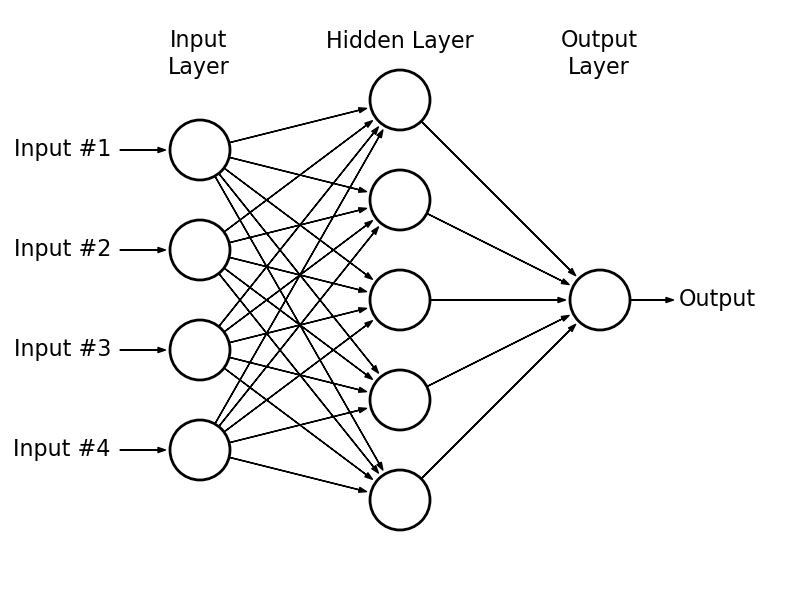
\includegraphics[width=\textwidth]{nn.png}
\caption{Basic example of a Neural Network, with a simple input, hidden and output layer. The Input Layer contain the split image(s), which then progress onto the Hidden layers. The output layer is a single neuron containing all the predictions made by the hidden layers.}
\end{subfigure}
\begin{subfigure}{0.6\textwidth}
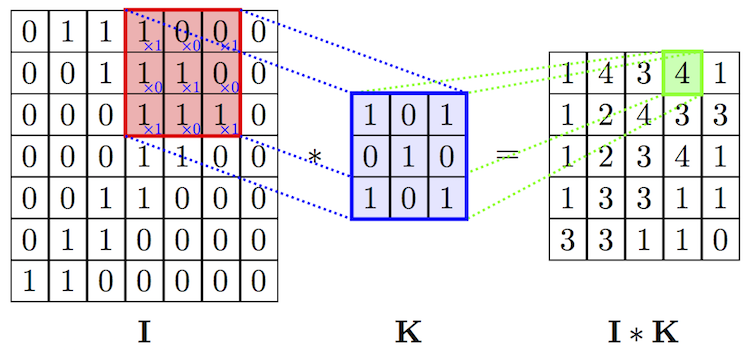
\includegraphics[width=\textwidth]{convolve.png}
\caption{Basic example of how a convolutional layer is created. A matrix dot function is applied to the layer (I) using a convolutional matrix (K); the resulting output layer is the matrix I*K.}
\end{subfigure}
\caption{Figures showing the basic layout of a Neural Network, (a), and a convolutional layer (b), found within the hidden layer of a network. All neurons within each layer connect to previous layers, as well as to future layers; as the layers 'learn', interaction strengths vary depending on how well each neuron classifies the data input into the model.}
\end{figure}

    
    By overlaying the kernel on top of the image in all possible ways, the convolutional layer is able to extract valuable information from the image, including edges and shape (\cite{zeiler_visualizing_2014}). This is process is aided by the non-linear activation functions applied to CNN layers, such as the ReLu function. These functions allow for true learning to take place, by allowing different input transformations to occur, which are learnt from the dataset itself (\cite{punjani_deep_2015}).


    Despite their excellent performance, CNNs require more resources in
    terms of computing power, as well as more time to train in comparison 
    to other machine learning algorithms (e.g., K-nearest neighbours, Random Forests). This 
    problem is further exacerbated because CNNs are difficult to design correctly, with many networks being created in the pursuit of the final model. Often, a balance must be struck between model factors (such as number of layers, layer type and parameters used) and the risk of over-fitting.

    Another commonly used algorithm in Plant Pathology is a Random Forest model (\cite{baranowski_hyperspectral_2015}). Despite returning lower accuracies than CNNs (\cite{baranowski_hyperspectral_2015}), they are still used and relied upon as a classifier; Ilastik (\cite{sommer_ilastik_2011}), an `interactive learning and segmentation toolkit', is developed in Python and utilisies Random Forest Classifiers. It is also a primary tool in classification in both Human and Plant Pathology (see: \cite{kleesiek_ilastik_2014, haubold_segmenting_2016,visschers_objective_2018}).

\subsection*{Image data}


Despite the excellent track records of Machine Learning alogrithms as image classifiers, the images used are still essential to creating a correctly classifying model. To ensure that the classifier does not overfit the data, images are often augmented prior to training (\cite{simard_best_2003, ciresan_high-performance_2011,ciresan_multi-column_2012,sladojevic_deep_2016}); the images are often augmented in such a way as to retain the structure of the image (i.e. transformations, rotations) whilst also providing additional test data. Images can also be normalised in an attempt to further reduce over-fitting and to allow comparison between datasets.



\begin{figure}[!t]
    \centering
    \begin{subfigure}[b]{0.3\textwidth}
        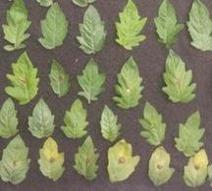
\includegraphics[width=\textwidth]{green.jpg}
        \caption{Dataset taken under RGB sensor \\ 
        }
  		\label{fig:sub1}
    \end{subfigure}
    \begin{subfigure}[b]{0.3\textwidth}
        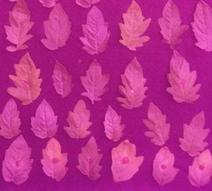
\includegraphics[width=\textwidth]{pink.jpg}
        \caption{Dataset taken under RGB sensor and CalColor 90 pink colour-pass filter}
  		\label{fig:sub2}
    \end{subfigure}
    \begin{subfigure}[b]{0.3\textwidth}
        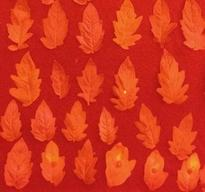
\includegraphics[width=\textwidth, height = 4.1cm]{red.jpg}
        \caption{Dataset taken under RGB sensor and CalColor 90 pink colour-pass filter}
  		\label{fig:sub2}
    \end{subfigure}
    \caption{Samples of dataset taken under different filters. Both b and c highlight chlorosis occuring in the leaves more evidently than in a.}
\label{fig:test}
\end{figure}

The quality of the image is also essential when it comes to building a classifier; Mou \textit{et al} (2017) note that hyperspectral imagery has started collecting considerable attention in the past few decades, in part due to it's high spectral resolution. Both multispectral and hyperspectral image data have been used in CNNs, and have achieved great results (\cite{harsanyi_hyperspectral_1994,delalieux_detection_2007,baranowski_hyperspectral_2015, zhu_early_2016, lowe_hyperspectral_2017,mou_deep_2017}). Although these methods have attracted attention over the recent decade, these imaging techniques are still costly. Another method for extracting valuable information from data are band-pass (Interference filters) and colour-pass filters (high pass filters; figure 2); these work by filtering image wavelengths, and allowing only specific wavelengths to pass whilst others are blocked. Band-pass filters are non-coloured and can allow very narrow wavelengths through; colour-pass filters are colured glass and work according to the principle of subtractive colour mixing (\cite{sischka_using_2018}). These filters allow for greater contrast within the image (Figure 2), and are gaining in popularity in image analysis (\cite{piron_selection_2008, knoth_unmanned_2013}).

\subsection*{Study - Organisms and Relevance/Outline }

Several methods are currently being used to study disease classification; more advanced models (\cite{zhu_early_2016}) are producing higher classification accuracies, and better quality images allow for additional information to be extracted (\cite{baranowski_hyperspectral_2015,lowe_hyperspectral_2017}). This paper will utilise both advanced models (CNNs and RFs), and high quality images produced using colour-pass filters.

This study will be classifying the impact of complex stresses on tomato (\textit{Solanum lycopersicum}) leaves; \textit{Botrytis cinerea}, a common fungal infection, and both drought and nitrogen deficiency were used as the stresses in this image dataset. A further study will look at the effect of infection duration on \textit{Arabadopsis thaliana}.

\textit{Arabadopsis thaliana} and Tomatoes were used as they are common study hosts in both host-pathogen and host-stress studies (\cite{tank_salinity-resistant_2010,singh_machine_2016,choi_positive_2017}); both have also been used in studies involving \textit{Botrytis cinerea} infection and resistance (\cite{diaz_role_2002,choi_positive_2017}).


\textit{Botrytis cinerea} is a commonly studied disease with distinguishable characteristics (\cite{awate_fruit_2015}); by using this fungal infection, we should obtain classifiable results, whilst also adding to the growing body of research in plant-host susceptibility and resistance. Finally, the abiotic stresses were chosen due to their notable effect on plant growth (drought:\cite{santos_path_2018}, nitrogen: \cite{zhao_nitrogen_2005}), and due to their ease of application. 


\subsection*{Aims of Project}


    This study was undertaken to see whether machine learning can correctly classify instances of complex stress 
    exposure in tomato leaves, as well as duration of infection of \textit{Botrytis cinerea} on \textit{Arabidopsis thaliana}.

    Our study aims to address five questions: Can machine learning classify instances of complex stress (question 1) and infection duration (question 2), will including colour-pass filtered images affect the model outcomes (question 3), will models trained on normalised images produce different results (question 4), and, will CNNs differ in model outcomes in comparison to RFs (qustion 5)?
    
    Based on previous studies looking into machine learning algorithms as plant disease classifiers (\cite{awate_fruit_2015,baranowski_hyperspectral_2015,sladojevic_deep_2016,singh_detection_2017,ubbens_deep_2017}), and on other image classification benchmarks that have been achieved using these algorithms (see:\cite{krizhevsky_imagenet_2012}), we believe both CNNs and RFs will be able to correctly classify (\textgreater 85\% training accuracy) both complex stresses (hypothesis 1) and infection duration (hypothesis 2) images. Including colour-pass filtered images should improve the classifiers accuracy (hypothesis 3); band-pass filters have already been used successfully in plant pathology (see: \cite{piron_selection_2008}) with colour-pass filters applying similar, but subtler, techniques. Models trained on the normalised dataset should have an improved accuracy rating in comparison to the original model accuracies (hypothesis 4); normalising the data should reduce the potential for over-fitting, and should also allow the model to be used on different datasets without requiring additional information. Due to the staggering performances of the top CNN models in many image classification challenges (for example, see: \cite{krizhevsky_imagenet_2012}), we also hypothesise that CNNs will produce better model outcomes in comparison to RFs (hypothesis 5).
    
\pagebreak    
  
\end{document}
   
   